\chapter{Approach}\label{sec:approach}

Two kind of approaches will be proposed. One one side, local approaches based on the PTAM implementation, where two steps are performed. The first step has been named \textit{Place Recognition} and the second \textit{Real Pose Recognition}. Multiple methods will be proposed to solve the second step. Then, on the other side, a global approach will be proposed. In this case machine learning methods (\textit{ferns}) will be used to recognize points in space.

\section{PTAM method}
\label{sec:ptam_method}

PTAM is a VO algorithm based on keyframes and so the relocalization method proposed is based on keyframes as well. Every keyframe has asociated with it a camera pose that will be used to relocalize. During the relocalization there are two steps involved. We have called the first step \textit{Place Recognition} and the second \textit{Real Pose Finder}.

\subsection{Place Recognition}
\label{ssub:place_recognition}

During this step, the algorithm tries to find the keyframe image most similar to the last acquired image. The pose associated with the most similar keyframe is used as an initial rough estimation of the current pose. The similarity score should be resistant to view point because the new acquired image will, most probably, never be taken from the same pose as any of the keyframes. Also it should be fast to compute.\\

The used similarity score is the Cross Correlation between images meaning the sum of the squared error between two zero-mean images. To make to computation faster both images are resized become $40\times30$. Then, to make the images more resistant to view point changes it is blurred with a $3\times3$ Gaussian kernel with $\sigma=2.5$. The resulting storied image is a resized, blurred and zero-mean image called \textit{small-blurry-image}.\\

During the normal map building pipeline this image is computed and stored every time a new keyframe is added to the map. And then, during the relocalization, the sum of squared difference between every stored \textit{small-blurry-image} and the last acquired frame is computed to find the most similar keyframe and then use its pose as an initial estimation of the current camera pose.\\

\subsubsection{Method evaluation}
\label{ssub:method_evaluation}

To evaluate the method the real distance between two frames is going to be compared with the Cross Correlation value described above. Far away frames should be dissimilar and close by frames should be more similar and have a lower CC value. In figure \ref{fig:real_distance_confusion_matrix} can be seen the pair distances between image using the real pose while in figure \ref{fig:CC_confusion_matrix} there is the approximated pair distances using the CC value as distance. It can be seen that they have a similar distribution. Also the correlation of 0.4337 shows that one explains the other in most cases.\\

\begin{figure}
  \begin{subfigure}[b]{0.60\linewidth}
          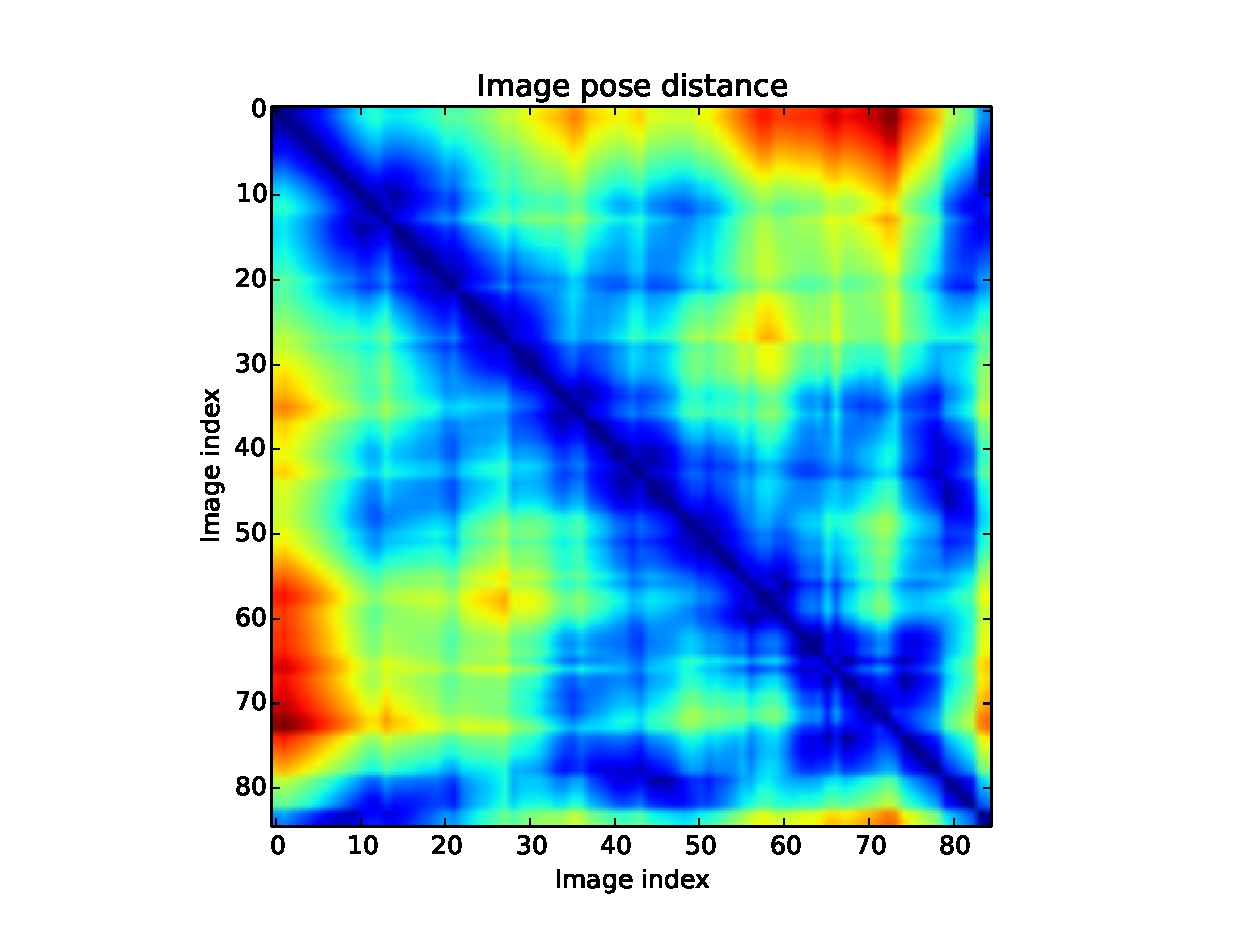
\includegraphics[width=\linewidth]{img/demo_1_1_CC_real_similarity_matrix.eps}
          \caption{Image to image real distance between the keyframe pose}                
          \label{fig:real_distance_confusion_matrix}
  \end{subfigure}   
  \qquad
  \begin{subfigure}[b]{0.60\linewidth}
         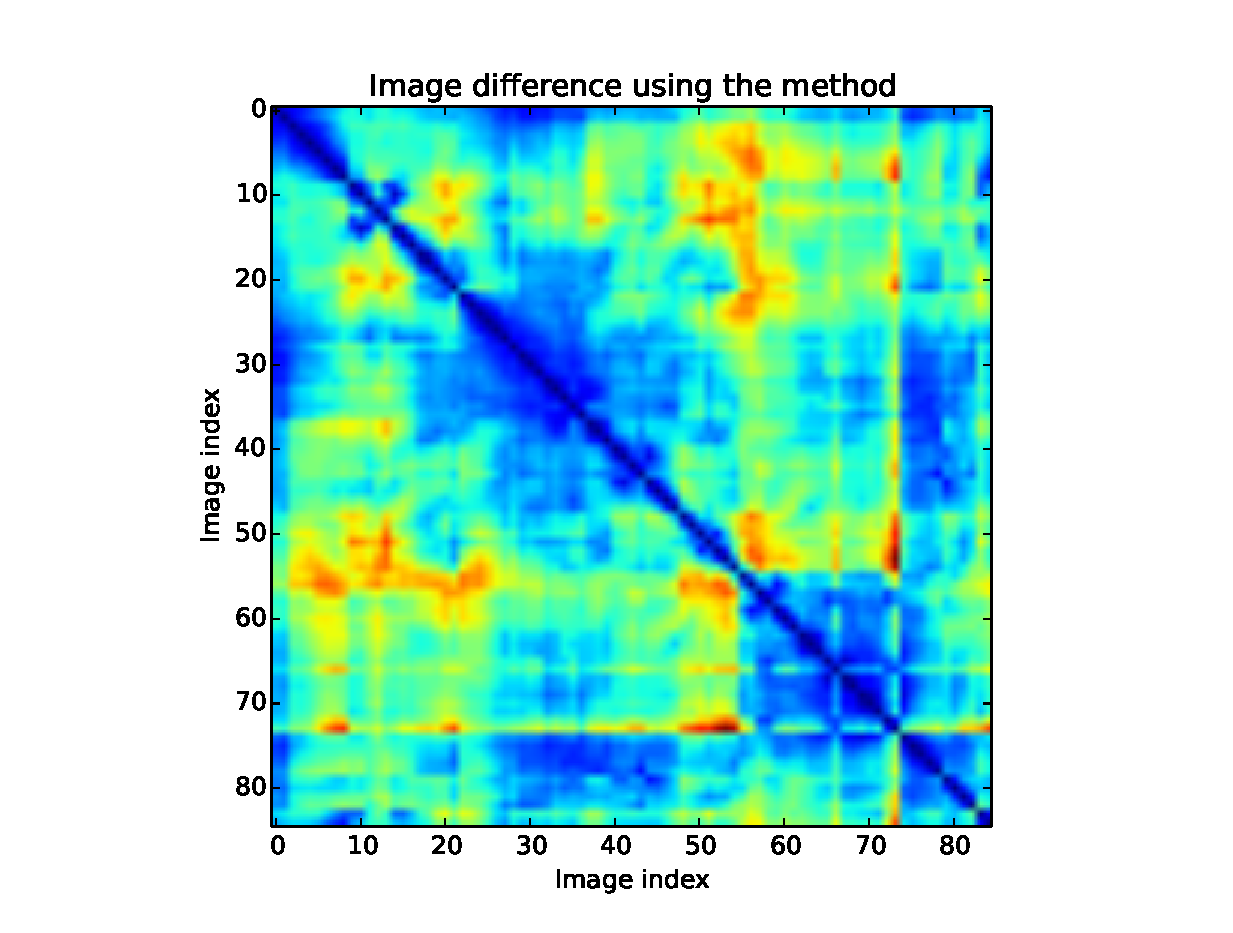
\includegraphics[width=\linewidth]{img/demo_1_1_CC_CC_similarity_matrix.eps}
         \caption{Image to image distance approximated using the Cross Correlation value}                
         \label{fig:CC_confusion_matrix}
  \end{subfigure}
  \caption{}
\end{figure}


Finally, to show that this method can be used, for every image the most CC similar image was taken being it real $K$ closest image. Ideally the most CC similar image should always be the closest image. In figure \ref{fig:K_closest} there is the count of occurrences of each $K$. It can be seen that most images resolve to the first or second closest image using this method.\\

\begin{figure}[!htbp]
  \centering
  \includegraphics[width=9cm]{img/demo_1_1_CC_choose_distribution.eps}
  \caption{}
  \label{fig:K_closest}
\end{figure}



\subsubsection{Real Pose Finder}
\label{ssub:real_pose_finder}

\chapter{To be removed}
\label{cha:chapter_name}



Describe the main steps in your algorithm. An illustration is always helpful.\\

Here are some \LaTeX~tips:


\section{Headings}

  Your report can be structured using several different types of headings. Use the commands \textbackslash\texttt{chapter}\{.\}, \textbackslash\texttt{section}\{.\}, \textbackslash\texttt{subsection}\{.\}, and \textbackslash\texttt{subsubsection}\{.\}. Use the asterisk symbol \texttt{*} to suppress numbering of a certain heading if necessary, for example, \textbackslash\texttt{section*}\{.\}.


\section{References}\label{sec:references}

  References to literature are included using the command \textbackslash\texttt{cite}\{.\}. For example \cite{KleinMurray2007,Strasdat2010WhyFilter}. Your references must be entered in the file \texttt{bibliography.bib}. Making changes or adding new references in the bibliography file can be done manually or by using specialized software such as \textit{JabRef} which is free of charge.

  Cross-referencing within the text is easily done using \textbackslash\texttt{label}\{.\} and \textbackslash\texttt{ref}\{.\}. For example, this paragraph is part of chapter~\ref{sec:approach}; more specifically on page~\pageref{sec:references}.

\section{Writing Equations}\label{sec:math}

  The most common way to include equations is using the \texttt{equation} environment. Use \textbackslash\texttt{eqref}\{.\} to reference an equation, e.g. \eqref{eq:leastsquares}.
  \begin{equation}\label{eq:leastsquares}
      \begin{aligned}
        C(\mathbf{x}) &= \frac{1}{2} \ \sum_{i \in \mathcal I} \sum_{k \in \mathcal K_i} \mathbf{e}_{i,k}(\mathbf{x})^T \ \mathbf{W}_{i,k}  \ \mathbf{e}_{i,k}(\mathbf{x})  \\
        \hat{\mathbf{x}}^{LS} &= \text{argmin}_\mathbf{x} \ C(\mathbf{x}),
      \end{aligned}
  \end{equation}

  \begin{equation}\label{eq:se3}
    \mathtt{T}_i = \begin{bmatrix}\mathbf{R}_i & \mathbf{p}_i \\ 0 & 1\end{bmatrix} \qquad \text{with} \quad \mathbf{R}_i \in SO(3), \ \ \mathbf{p} \in \mathbb{R}^3.
  \end{equation}

\section{Including Graphics}\label{sec:epsgraph}
  The easiest way to include figures in your document is to use pdf figures if you use \texttt{pdflatex} to compile. Figure \ref{img:notation} was created with the use of the open source program \texttt{ipe}.

  \begin{figure}[h]
     \centering
     \includegraphics[width=0.6\textwidth]{img/notation.pdf}
     \caption{Example of a figure.}
     \label{img:notation}
  \end{figure}


\section{Including Code in your Document}

  You may include samples from your Matlab code using the \texttt{lstlistings} environment, for example
  \lstset{language=Matlab,numbers=none}
  \begin{lstlisting}[frame=lines, caption=Matlab Example, label=matlabexample]
  % Evaluate y = 2x
  for i = 1:length(x)

    y(i) = 2*x(i);

  end
  \end{lstlisting}

  \lstset{language=C++,numbers=none,caption=C++ Example, label=cppexample}
  \begin{lstlisting}[frame=lines]
  % sum all elements in a list
  int sum=0;
  for(list<int>::iterator it=mylist.begin(); it!=mylist.end(); ++it)
    sum += *it;
  \end{lstlisting}
